\documentclass{tudelft-report}

%% Set up the bibliography
\usepackage{biblatex}
\usepackage[utf8]{inputenc}
\usepackage{enumitem} 
\usepackage{titlesec} % For title formatting
\usepackage{comment}
\usepackage{tabularx}
\usepackage{float}
\usepackage{hyperref}
\usepackage[l3]{csvsimple}
\addbibresource{report.bib}

%% Additional packages and commands
\usepackage{parskip}
\setlist{itemsep=-2pt} % Reducing white space in lists slightly
\renewcommand{\deg}{\si{\degree}\xspace} % Use \deg easily, everywhere

\titlespacing*{\section}
{0pt}{4.0ex plus 1ex minus .2ex}{2.2ex plus .2ex}
\titlespacing*{\subsection}
{0pt}{3.5ex plus 1ex minus .2ex}{1.8ex plus .2ex}
\titlespacing*{\subsubsection}
{0pt}{3.0ex plus 1ex minus .2ex}{1.5ex plus .2ex}

\usepackage{hyperref}
\hypersetup{
    colorlinks=true,
    linkcolor=blue,
    filecolor=magenta,      
    urlcolor=cyan,
    pdftitle={Overleaf Example},
    pdfpagemode=FullScreen,
    }

\urlstyle{same}

% Define the instruction box style
\specialcomment{instruction}{\begingroup\color{red}\itshape}{\endgroup}
\excludecomment{instruction} % Exclude all instructions from printing

%% ----------------------------------------------------------------------
%%    Begin of document + Frontmatter (Roman page numbering)
%% ----------------------------------------------------------------------

\begin{document}

\frontmatter

%% Define the main parameters
\title{IOF Core Patterns}
\subtitle{A compendium of Semantic Data Patterns based on IOF Core}
\author{Author1 \\ Author2}

\subject{Draft} % Cover only
\affiliation{NIST} % Cover only
\coverimage{figures/College-Cover-Page.pdf} % Aspect ratio of 2:3 (portrait) recommended
\definecolor{title}{HTML}{fee7dd} % Color for cover title

% \makecover

\begin{titlepage}

\begin{center}

%% Print the title
{\makeatletter
\largetitlestyle\fontsize{45}{45}\selectfont\@title
\makeatother}

%% Print the subtitle
{\makeatletter
\ifdefvoid{\@subtitle}{}{\bigskip\titlestyle\fontsize{20}{20}\selectfont\@subtitle}
\makeatother}

\bigskip
\bigskip

by

\bigskip
\bigskip

%% Print the name of the author
{\makeatletter
\largetitlestyle\fontsize{25}{25}\selectfont\@author
\makeatother}

\bigskip
\bigskip

%% Print table with names; easily add columns if necessary or remove the table completely
\setlength\extrarowheight{2pt}
% \begin{tabular}{l}
    % Editor: TBD \\\midrule
    % Contributors: TBD  \\
% \end{tabular}

\vfill

%% Print some more information at the bottom
\begin{tabular}{ll}
    Authors: & I. Surname \\
    Editors: & I. Surname \\
    Proofread by: &  I. Surname1, I. Surname2
\end{tabular}

\bigskip
\bigskip

%% Add a source and description for the cover and optional attribution for the template
\begin{tabular}{p{15mm}p{10cm}}
    Copyright: & (c) 2025, Open Applications Group   \\
    % Feel free to remove the following attribution, it is not required - still appreciated :-)
    Release:  & 2025
\end{tabular}

\end{center}

%% Insert the TU Delft logo at the bottom of the page
\begin{tikzpicture}[remember picture, overlay]
    \node[above=10mm] at (current page.south) {%
        \includegraphics[scale=0.3]{figures/OAGi-IOF.png}
    };
\end{tikzpicture}

\end{titlepage}

\input{frontmatter/preface}
\chapter*{Summary}
\addcontentsline{toc}{chapter}{Summary}

summary of the compendium ...










\tableofcontents
%\listoffigures
%\listoftables

\chapter*{Glossary}
\addcontentsline{toc}{chapter}{Glossary}

\emph{List all domain-specific, technical, other abbreviations and internally standardised terms in the glossary, e.g., construct - we mean terms in IOF. \\ 
DO NOT include ontology constructs including BFO or IOF in the glossary.}

\noindent
\setlist[description]{style=nextline, labelwidth=0pt, leftmargin=1.5em, labelsep=0.9em} % Customize hanging indent
\begin{description}
    \item[\textbf{aliquam}] 
    \hspace{3mm} tincidunt urna. Nulla ullamcorper vestibulum turpis. Pellentesque cursus luctus mauris.
    
    \item[\textbf{cras viverra}]
    \hspace{3em} metus rhoncus sem. Nulla et lectus vestibulum urna fringilla ultrices. Phasellus eu tellus sit amet tortor gravida placerat.
    
    \item[\textbf{donec nonummy}]
    \hspace{3em} pellentesque ante. Phasellus adipiscing semper elit. Proin fermentum massa ac quam. Sed diam turpis, molestie vitae, placerat a, molestie nec, leo.
    
    \item[\textbf{integer sapien}]
    \hspace{3em} est, iaculis in, pretium quis, viverra ac, nunc. Praesent eget sem vel leo ultrices bibendum. Aenean faucibus.
    
    \item[\textbf{lorem ipsum}]
    \hspace{3em} dolor sit amet, consectetur adipiscing elit. Ut purus elit, vestibulum ut, placerat ac, adipiscing vitae, felis. Curabitur dictum gravida mauris.
\end{description}




%% ----------------------------------------------------------------------
%%    Mainmatter (Arabic page numbering)
%% ----------------------------------------------------------------------

\mainmatter

\chapter{Introduction}
\label{chapter:introduction}
% Instruction box
\textit{
This chapter is for everything we need to inform in general before presenting the patterns.
}


\section*{Purpose and scope}
\addcontentsline{toc}{section}{Purpose and scope}

\section*{Basic Formal Ontology (BFO)}
\addcontentsline{toc}{section}{Basic Formal Ontology}

\section*{IOF Core}
\addcontentsline{toc}{section}{IOF Core}


\section*{How to use the patterns}
\addcontentsline{toc}{section}{How to use the patterns}

\subsection*{Identify the correct patterns to use}
\addcontentsline{toc}{section}{Identify the correct patterns to use}


\subsection*{Use in Data mapping}
How to use the INSERT DATA mapping (adopt and adjust) 

\subsection*{Use in Data validation}
SPARQL and SHACL

\subsection*{Extension and customization}
understand the general pattern
Explore how different patterns can be combined.

\section*{Versioning and changes}


%\input{mainmatter/chapter-4} % Create file to add

%% ----------------------------------------------------------------------
%%    Aspects and scenerios
%% ----------------------------------------------------------------------
\textit{
Only add aspects that are main chapters. Each scenario will be a section with TOC entry only with the scenario name. Compile scenarios under the aspect chapters below.
}

\input{mainmatter/space-location}
\chapter{Time}

\section{Clock time and calendar date}
\label{sec-change-location}

\textbf{Created by:} Arkopaul Sarkar \\
\textbf{Modified by:} Arkopaul Sarkar \\

\subsection*{Scenario Objective}

This scenario illustrates how to associate clock time and calendar dates with the instances of time. While the ability to store the clock time and calendar date lets the users perform various quantitative analyses on the processes and their durations, a wide variety of clock and calendar systems makes it challenging to represent the date and times in the correct format. We include use cases depicting basic to advanced methods of representing date and time values of the temporal instances.


\subsection*{General Pattern Description}

\includegraphics[scale=0.28]{scenarios/clock-time-calendar-date/images/general-clock-calendar.png}

the calendar and clock time for a specific temporal instant can be expressed by associating different instances of the information class \texttt{TemporalInstantValueExpression} or OWL-Time class \texttt{time:General\\DateTimeDescription} as both are subclass of \texttt{time:TemporalPosition} (\texttt{core:TemporalInstantValue\\Expression} is mapped as subclass of \texttt{time:TemporalPosition}.  

\subsubsection*{Use Case: Launch of first iPhone} 
The original iPhone was first launched on June 29, 2007 during the Macworld Conference \& Expo in San Francisco, California. 

The date and time of the launch are captured in 1) XSD dateTime format, 2) in a specific time zone, and 3) using a custom date and time format. The process \texttt{launch-of-iphone} is not detailed further except the temporal interval it occupies. This instance of temporal interval is then connected to its first temporal instant, for which the calendar date and clock time are assigned.   

\subsubsection*{Use-Case Pattern Description}

\includegraphics[scale=0.35]{scenarios/clock-time-calendar-date/images/uc1-dow-mn.png}

The launch date and time are expressed in three different ways.  

\texttt{hasDateTimeInstantValue} can associate the date and time value in \texttt{xsd:dateTime} format. If the date and time values can be expressed in XSD format, this pattern does not require any reference to OWL Time ontology. Also, \texttt{xsd:dateTime} format already has provision for mentioning time zone (e.g., 2007-06-29T18:00:00-05:00 for a UTC-5 timezone). However, as XSD:dateTime datatype is the range of \texttt{hasDateTimeInstantValue}, no other XSD type or a different format can be expressed using this pattern. 

\paragraph{Other components of a clock time \\}

In the above pattern, the launch date and time of the iPhone in New York are expressed as `day of the week' using \texttt{time:dayOfWeek} (OWL Time ontology provides the days of a week as instances of type \texttt{time:DayOfWeek})  and `month', using \texttt{time:month} data property \texttt{xsd:gMonth} which links to an indexical value based on the order of months in the calendar of type \texttt{xsd:gMonth} \footnote{\url{https://www.w3.org/TR/xmlschema11-2/\#gMonth}}.
Various combinations of data properties of \texttt{GeneralisedDateTimeDescription}, e.g.,  year, month, day, hour, minute, and second, can be used to express a clock time or calendar date, e.g., only date value in year, month and day. The corresponding time zone can be mentioned by linking an instance of \texttt{TimeZone} \footnote{For detailed guidance about working with time zones, see \url{http://www.w3.org/TR/timezone/} .}, using \texttt{time:timeZone} property.       

\paragraph{Using custom clock time format \\}

\includegraphics[scale=0.35]{scenarios/clock-time-calendar-date/images/uc1-custom.png}

In the above pattern the launch date is expressed in `GPS time'. As GPS time is the number of seconds since an epoch in 1980, encoded as the number of weeks and seconds into the week, the new class  \texttt{GPSTimeDescription}, extended from \texttt{time:DateTimeDescription}, should contain values for data properties \texttt{time:second} and \texttt{time:week}. The example does not provide details of \texttt{GPSTimeSystem}, which is a \texttt{time:TemporalReferenceSystem}, and may refer to a suitable description of `GPS time', e.g., A taxonomy of temporal reference systems is provided in ISO 19108:2002. 


\subsubsection*{Data Mapping Description}

\begin{verbatim}
INSERT DATA {
    ns1:launch-of-iphone a bfo:Process;
                        bfo:occupiesTemporalRegion ns1:launch-interval.
    ns1:launch-interval a bfo:TemporalInterval;
                        iof:hasFirstInstant ns1:launch-start-time.
    ns1:launch-start-time a bfo:TemporalInstant;
                        iof:hasValueExpressionAtAllTimes ns1:instant-expression-xsd;
                        iof:hasValueExpressionAtAllTimes ns1:instant-expression-month;
                        iof:hasValueExpressionAtAllTimes ns1:instant-expression-dow;
                        iof:hasValueExpressionAtAllTimes ns1:instant-expression-gps.
    ns1:instant-expression-xsd a iof:TemporalInstantValueExpression;
                        iof:hasDateTimeInstantValue "2007-06-29T18:00:00Z"^^xsd:dateTime.
    ns1:instant-expression-month a time:DateTimeDescription;
                        time:month "--06"^^xsd:gMonth.
    ns1:instant-expression-dow a time:DateTimeDescription;
                        time:dayOfWeek time:Friday.
    ns1:instant-expression-gps a ns:GPSTimeDescription;
                        time:week "1430"^^xsd:decimal;
                        time:second "324018"^^xsd:decimal. 
}
\end{verbatim}


\subsubsection*{Data Validation}



\section{Duration in time units}
\label{sec-change-location}

\textbf{Created by:} Arkopaul Sarkar \\
\textbf{Modified by:} Arkopaul Sarkar \\

\subsection*{Scenario Objective}

This scenario demonstrates how to represent time durations of time intervals. Duration values can be measured in different time units, such as years, hours, and ticks. In the following, we present the patterns for asserting duration values in standard and custom units.   

\subsection*{General Pattern Description}

\includegraphics[scale=0.36]{scenarios/time-duration/image/time-duration.png}

The duration of a temporal interval can be expressed by associating different instances \texttt{iof:TemporalDurationValueExpression} or some subtype of OWL-Time class \texttt{time:TemporalDuration} to the instance of \texttt{bfo:TemporalInterval} using \texttt{iof:isValueExpressionOfAtAllTimes} as they are equivalent classes. An instance of \texttt{time:DurationDescription}, which is a subclass of \texttt{time:TemporalDuration}, provides several data properties to assert the duration value in various units used in Gregorian Calendar, e.g., \texttt{time:years}, \texttt{time:months}, and \texttt{time:minutes}. Alternatively, a numeric value and corresponding duration type can be asserted using the instance of \texttt{time:Duration}. A custom duration description class can be defined by extending \texttt{time:GeneralDurationDescription} class with an appropriate temporal reference system. 

\subsubsection*{Use Case: Duration of OntoCommons project} 
OntoCommons project started on Wednesday, 1 September 2021 and ended on Saturday, 9 November 2024. It ran for 1165 days from the start date to the end date, not including the end date.

The date and time of the launch are captured in 1) XSD dateTime format, 2) in a specific time zone, and 3) using a custom date and time format. The process \texttt{launch-of-iphone} is not detailed further except the temporal interval it occupies. This instance of temporal interval is then connected to its first temporal instant, for which the calendar date and clock time are assigned.   

\subsubsection*{Use-Case Pattern Description}

\includegraphics[scale=0.35]{scenarios/time-duration/image/uc1}

The launch date and time are expressed in three different ways.  

\texttt{hasDateTimeInstantValue} can associate the date and time value in \texttt{xsd:dateTime} format. If the date and time values can be expressed in XSD format, this pattern does not require any reference to OWL Time ontology. Also, \texttt{xsd:dateTime} format already has provision for mentioning time zone (e.g., 2007-06-29T18:00:00-05:00 for a UTC-5 timezone). However, as XSD:dateTime datatype is the range of \texttt{hasDateTimeInstantValue}, no other XSD type or a different format can be expressed using this pattern. 

\includegraphics[scale=0.35]{scenarios/clock-time-calendar-date/images/uc1-dow-mn.png}

\paragraph{Other components of a clock time \\}

In the above pattern, the launch date and time of the iPhone in New York are expressed as `day of the week' using \texttt{time:dayOfWeek} (OWL Time ontology provides the days of a week as instances of type \texttt{time:DayOfWeek})  and `month', using \texttt{time:month} data property \texttt{xsd:gMonth} which links to an indexical value based on the order of months in the calendar of type \texttt{xsd:gMonth} \footnote{\url{https://www.w3.org/TR/xmlschema11-2/\#gMonth}}.
Various combinations of data properties of \texttt{GeneralisedDateTimeDescription}, e.g.,  year, month, day, hour, minute, and second, can be used to express a clock time or calendar date, e.g., only date value in year, month and day. The corresponding time zone can be mentioned by linking an instance of \texttt{TimeZone} \footnote{For detailed guidance about working with time zones, see \url{http://www.w3.org/TR/timezone/} .}, using \texttt{time:timeZone} property.       

\paragraph{Using custom clock time format \\}

\includegraphics[scale=0.35]{scenarios/clock-time-calendar-date/images/uc1-custom.png}

In the above pattern the launch date is expressed in `GPS time'. As GPS time is the number of seconds since an epoch in 1980, encoded as the number of weeks and seconds into the week, the new class  \texttt{GPSTimeDescription}, extended from \texttt{time:DateTimeDescription}, should contain values for data properties \texttt{time:second} and \texttt{time:week}. The example does not provide details of \texttt{GPSTimeSystem}, which is a \texttt{time:TemporalReferenceSystem}, and may refer to a suitable description of `GPS time', e.g., A taxonomy of temporal reference systems is provided in ISO 19108:2002. 


\subsubsection*{Data Mapping Description}

\begin{verbatim}
INSERT DATA {
    ns1:ontocommons-project a bfo:Process ;
                             bfo:occupiesTemporalRegion ns1:oc-project-interval .

    ns1:oc-project-interval a bfo:TemporalInterval .

    ns1:oc-project-duration1 a time:DurationDescription ;
                              iof:isValueExpressionOfAtAllTimes ns1:oc-project-interval ;
                              time:years "3"^^xsd:decimal ;
                              time:months "8"^^xsd:decimal ;
                              time:days "2"^^xsd:decimal .

    ns1:oc-project-duration2 a time:Duration ;
                              iof:isValueExpressionOfAtAllTimes ns1:oc-project-interval ;
                              time:numericDuration "1165"^^xsd:decimal ;
                              time:unitType time:unitDay .

    ns1:oc-project-duration3 a ns:FiscalQuarter ;
                              iof:isValueExpressionOfAtAllTimes ns1:oc-project-interval ;
                              ns:fiscalQuarters "12"^^xsd:decimal .
}
\end{verbatim}

\texttt{ns:GPSTimeDescription} class has a temporal reference system as \texttt{ns:GPSTimeSystem}, which refer to the specification of GPS time format. Following the standard, a \texttt{GPSTimeDescription} has a 

\begin{verbatim}
:GPSTimeDescription rdf:type owl:Class ;
    rdfs:subClassOf 
    <http://www.w3.org/2006/time#GeneralDateTimeDescription> ,
    [ rdf:type owl:Restriction ;
        owl:onProperty <http://www.w3.org/2006/time#hasTRS> ;
        owl:hasValue :GPSTimeSystem
    ] ,
    [ rdf:type owl:Restriction ;
        owl:onProperty <http://www.w3.org/2006/time#unitType> ;
        owl:hasValue <http://www.w3.org/2006/time#unitSecond>
    ] .    

:GPSTimeSystem rdf:type owl:NamedIndividual ,
    <http://www.w3.org/2006/time#TRS> ;
    AnnotationVocabulary:adaptedFrom "https://en.wikipedia.org/?title=GPS_time" .
\end{verbatim}


\subsubsection*{Data Validation}


\chapter{Objects, artifacts and their materials}

\section{object vs artifact}
\section{What an Object is Made of}
\label{chapter-scenario-template}
\textit{This template should be used to create a scenario. Please copy to a dedicated folder under folder `scenario'. All images should be referred from `image' folder under the dedicated folder. For example, please see: \\
\cref{sec-change-location}}

\section*{<Scenario title>}


\textbf{Created by:} Perawit Charoenwut \\
\textbf{Modified by:} Perawit Charoenwut \\

\subsection*{Scenario Objective}


\subsection*{General Pattern Description}





\subsection*{Use Case: <Use-Case title>}

\subsubsection*{Use-Case Pattern Description}

\subsubsection*{Use-Case Example Data}


\subsubsection*{Data Mapping}


\subsubsection*{Data Validation}


\section{material vs object}


\section{material vs material constitution}


\section{object vs fiat objects}


\section{part of an object}

\chapter{Assembly component}

\section{components of an assembly}
\section{Assembly component}

\textbf{Created by:} Dušan Šormaz \\
\textbf{Modified by:}  \\

address all times/ sometimes and also transitivity of these two pairs of relationships.

\subsection*{Scenario Objective}
From Arko's email, 1/7/25 
I want to mention that however we are showing the basic use of "component part of" relation for expressing parthood, we should also show the use of "at some time" vs. "at all times" under this scenario. Also, the nuanced semantics of "component of at all times" vs. "has component at all times" (explain why they are not inverses to each other) is to be examined.
DNS
We also need to show multiple levels of assemblies, at least three. Should we consider assembly process(es)?
\subsection*{General Pattern Description}
This scenario shows uses of \texttt{iof:componetPartOf}, \texttt{bfo:continuantPartofAtSomeTime}, and \texttt{bfo:continuantPartofAtAllTimes} object properties. The general pattern is shown in fig. 

\begin{figure}
\includegraphics[scale=0.5]{scenarios/object-artifact-material/image/what-is-made-of.png}
\caption{The general pattern for the use of component related object properties} 
\label{gen-pttn-components}
\end{figure}


\subsection*{Examples}

A car engine is often showcased in parts: pistons, crankshaft, and cylinders.

An insulated wall comprises drywall, insulation foam, and outer sheathing.

Sewing patches of silk, cotton and leather make an item of clothing.

\section{Embedded components}

Reinforcement Bars in Concrete Structures

coating on a metal surface - this is not assembly

printed circuit on board

Embedded sensors


\section{being components of different assemblies at different times}

\textbf{Created by:} Ali Hasanzadeh \\
\textbf{Modified by:}  \\

\subsection*{Scenario Objective}

This scenario illustrates how to represent the change in an object's association with different assemblies over time using the IOF/BFO ontology framework. It focuses on:
\begin{itemize}
    \item Highlighting the use of temporal regions and temporal intervals to associate an object's presence in specific assemblies over time.
    \item Representing the object's changing relationships to multiple assemblies through different parthood properties.
    \item Using physical connections of components as an outcome some process assembly to denote a material artifacts function(s). 
\end{itemize}

\subsection*{General Pattern Description}

\includegraphics[scale=0.48]{scenarios/assemblies-components/images/assembly-component-general-pattern-description.png}

A material component may be a component of different assemblies at different times. In this scenario, the \texttt{core:MaterialComponent} would be related to multiple \texttt{core:Assembly} via the \texttt{core:componentPartOfAtSomeTime} property. As this connection cannot be true between a \texttt{core:MaterialComponent} and different \texttt{core:Assembly} artifacts at once, we would denote this reality by pairing the \texttt{bfo:TemporalRegion} of each \texttt{core:AssemblyProcess} with the \texttt{core:MaterialComponent}.

\subsection*{Use-Case Pattern Description}
A PLA joint can be part of a modular shelf used for storing books and later be repurposed in another modular shelf used for storing tools. The particular example is chosen to emphasize the difference between assemblies and machines as well. In this scenario, the joint is \texttt{core:componentPartOfAtSomeTime} multiple shelves (\texttt{core:Assembly}). In other words, this \texttt{core:Component} is \texttt{core:componentPartOfAtSomeTime} one \texttt{core:Assembly} shelf at some \texttt{bfo:TemporalRegion} as the result of some \texttt{core:AssemblyProcess} and \texttt{core:componentPartOfAtSomeTime} of another \texttt{core:Assembly} shelf at some other \texttt{bfo:TemporalRegion} as the result of a different \texttt{core:AssemblyProcess}.

\section{being components of different assemblies at the same times}

door is a component of both room.

\section{Temporary components}

Each stage of the rocket is only part of the whole vehicle for a specific phase of the journey

\section {Components as an identity of the assembly}

Changing the battery of a wall clock or the tire of a car does not change the wall clock or the car.

But changing the CPU changes the laptop. 









\chapter{Person and agent}

Agent as an organisational agent

Agent as a group of agents 

Agent as an EngineeredSystem
\chapter{System and organization}

\section{Different types of organisations}
\label{chapter-scenario-template}
\textbf{Created by:} Perawit Charoenwut \\
\textbf{Modified by:}

\subsection*{Scenario Objective}
This scenario illustrates how to represent a complete company structure with manufacturing and business divisions using the IOF core ontology. It focuses on:
\begin{itemize}
    \item Showing how business and manufacturing units coexist within one company
    \item Representing organizational hierarchy and relationships
    \item Distinguishing between business and manufacturing activities
    \item Capturing different organizational roles and functions
\end{itemize}

\subsection*{General Pattern Description}
A company can contain both business organizations and manufacturers as part of its structure. While all are types of Organization, they serve different functions and have different activities within the company structure.
\includegraphics[scale=0.5]{scenarios/object-artifact-material/image/}


\subsection*{Use Case: }
A comprehensive example using a car company structure, which includes both manufacturing plants and business divisions.

\subsubsection*{Use-Case Pattern Description}
The company structure includes:
\begin{itemize}
    \item Parent company (Organization)
    \item Regional business divisions (BusinessOrganization)
    \item Manufacturing plants (Manufacturer)
    \item Sales and service divisions (BusinessOrganization)
\end{itemize}

\subsubsection*{Use-Case Example Data}
\begin{table}[h]
% \caption{}
\label{tab:organization-structure}
\resizebox{\columnwidth}{!}{%
\begin{tabular}{|l|l|l|l|l|}
\hline
Org\_ID & Org\_Type & Primary\_Activity & Functions \\ \hline
C\_001 & Organization & Corporate Management & Strategic Planning, Governance \\
M\_001 & Manufacturer & Vehicle Manufacturing & Assembly, Quality Control, R\&D \\
M\_002 & Manufacturer &  Parts Manufacturing & Parts Production, Testing \\
S\_001 & BusinessOrg &  Vehicle Sales & Marketing, Dealership Management \\
F\_001 & BusinessOrg &  Financial Services & Leasing, Insurance, Loans \\
L\_001 & BusinessOrg & Logistics Services & Transportation, Distribution \\ \hline
\end{tabular}%
}
\end{table}


\subsubsection*{Data Mapping}


\subsubsection*{Data Validation}


\section{System and subsystem}





\chapter{Role}

\section{Gain and loss of roles}

\textbf{Created by:} Arkopaul Sarkar \\
\textbf{Modified by:} Arkopaul Sarkar \\

\subsection*{Scenario Objective}

BFO roles are realizable entities external to the bearer and assigned within specific physical, social, or institutional contexts. A bearer can hold multiple roles over time or simultaneously, without ceasing to exist when roles change. However, BFO lacks constructs to indicate when roles begin or end. This scenario discussed the patterns around two subclasses of bfo:process, introduced by IOF Core to represent the the start and end of role. 

\subsection*{General Pattern Description}


\begin{figure}[ht]
    \centering
    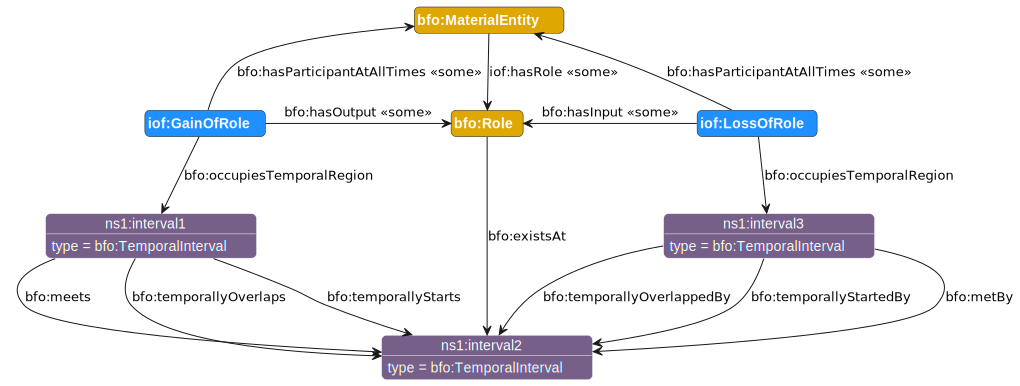
\includegraphics[scale=0.35]{scenarios/role-gain-loss/images/general-pattern.png}
    \label{fig:role-gain-loss-gp}
\end{figure}

Being specifically dependent continuants, BFO roles inheres in some independent containuant except spatial regions. The generic pattern diagram shows only material entity which bears the role (IOF provides a specialized property `has role' to only assign role to an entity) but some immaterial entities, such as sites and boundaries may also have a role. 

An intuitive way time bound the role is to use BFO `exists at' relation which links a temporal region to any entity. However, there is no constraints in BFO or IOF to obligate the role to be assigned to only one bearer during its existence, however, that may be the best practice. Moreover, the assignment and removal of a role from an entity may not have a sharp time point, e.g., an operator may need to go through a period of training to actually receive the role, or a product may need to go through testing and validation after it is bought and before it is registered as an asset (asset role) of the organization. Gain and loss of role classes provide user a way to assert actual start and end of a material entity carries a role. 

It can be noted that both `gain of role' and `loss of role' are BFO process, which signifies the processes of a material entity gaining and losing a role. The material entity bearing the role participates in these processes and the role it bears is the output of the gain-of-role process, and input of the loss-of-role process. Msot importantly, the interval for which the gain-of-role process occurs may meet, overlap, or start the interval for which the material entity bears the role and, conversely, the interval for which the loss-of-role process occurs may be met by, overlapped by, or started by the interval for which the material entity bears the role. This implies that the material entity may start bearing the role as soon as the process of gaining the role starts, or starts right after the role is gained, or somewhat in between. Similary, the material entity may stop bearining the role at the start of the losing the role process, or at the end of it, or somewhat in between. The user may select any combination of the above temporal relations depending on their requirements to assert the duration of the role. Some of these choices are explained in the use cases. 


\subsection*{Use Case: Assignment and Removal of a Safety Officer}

John K. Lee was appointed as the Safety Officer by the HR department of a manufacturing business on May 1, 2024. Following this decision, his role was formally registered in the company’s HR system on May 3, 2024. He officially began his duties at Plant A on May 6, 2024, taking on responsibilities related to workplace safety and compliance.

After serving in the role for nearly ten months, the HR department initiated the termination process of his appointment on March 31, 2025, upon completion of the planned term. Due to routine administrative handling, the role was formally deactivated in the system on April 4, 2025, which also marked John’s last working day as Safety Officer. He returned to his prior position thereafter.

\subsubsection*{Use-Case Pattern Description}

\begin{figure}[ht]
    \centering
    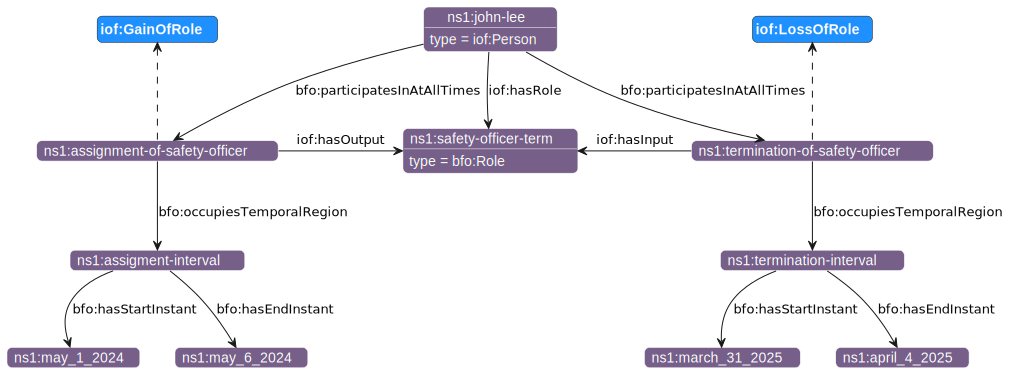
\includegraphics[scale=0.35]{scenarios/role-gain-loss/images/use-case1.png}
    \label{fig:role-gain-loss-gp}
\end{figure}

\subsubsection*{Data Mapping}

\begin{verbatim}
PREFIX xsd: <http://www.w3.org/2001/XMLSchema#>
PREFIX rdf: <http://www.w3.org/1999/02/22-rdf-syntax-ns#>
PREFIX ns1: <http://example.org/ns1#>
PREFIX bfo: <http://purl.obolibrary.org/obo/> 
PREFIX iof: <https://spec.industrialontologies.org/ontology/core/Core/>

INSERT DATA {
    
    ns1:john-lee a iof:Person;
    	bfo:BFO_0000166 ns1:assignment-of-safety-officer;
    	bfo:BFO_0000166 ns1:termination-of-safety-officer;
    	iof:hasRole ns1:safety-officer.
    
    ns1:safety-officer a bfo:BFO_0000023.

    ns1:assignment-of-safety-officer a iof:GainOfRole;
        bfo:occupiesTemporalRegion ns1:assignment-interval;
    	iof:hasOutput ns1:safety-officer.

    ns1:assignment-interval a bfo:BFO_0000202;
        bfo:BFO_0000222 ns1:assignment-start-time;
        bfo:BFO_0000224 ns1:assignment-end-time.
    
    ns1:assignment-start-time a bfo:BFO_0000203;
        iof:hasValueExpressionAtAllTimes ns1:assignment-start-time-value.

    ns1:assignment-end-time a bfo:TemporalInstant;
        iof:hasValueExpressionAtAllTimes ns1:assignment-end-time-value. 

    ns1:assignment-start-time-value iof:hasDateTimeInstantValue "2024-05-01T00:00:00Z"^^xsd:dateTime.
    ns1:assignment-end-time-value iof:hasDateTimeInstantValue "2024-05-06T00:00:00Z"^^xsd:dateTime.

    ns1:termination-of-safety-officer a iof:LossOfRole;  
        bfo:occupiesTemporalRegion ns1:termination-interval;
    	iof:hasInput ns1:safety-officer.

    ns1:termination-interval a bfo:BFO_0000202;
        bfo:BFO_0000222 ns1:termination-start-time;
        bfo:BFO_0000224 ns1:termination-end-time.
    
    ns1:termination-start-time a bfo:BFO_0000203;
        iof:hasValueExpressionAtAllTimes ns1:termination-start-time-value.

    ns1:termination-end-time a bfo:TemporalInstant;
        iof:hasValueExpressionAtAllTimes ns1:termination-end-time-value. 

    ns1:termination-start-time-value iof:hasDateTimeInstantValue "2025-03-31T00:00:00Z"^^xsd:dateTime.
    ns1:termination-end-time-value iof:hasDateTimeInstantValue "2025-04-04T00:00:00Z"^^xsd:dateTime.
}

\end{verbatim}

\subsubsection*{Data Validation}

\begin{verbatim}
PREFIX xsd: <http://www.w3.org/2001/XMLSchema#>
PREFIX rdf: <http://www.w3.org/1999/02/22-rdf-syntax-ns#>
PREFIX sh:  <http://www.w3.org/ns/shacl#>
PREFIX ns1: <http://example.org/ns1#>
PREFIX bfo: <http://purl.obolibrary.org/obo/> 
PREFIX iof: <https://spec.industrialontologies.org/ontology/core/Core/>
PREFIX ex:  <http://example.org/shapes#>

ex:AssignmentEventShape a sh:NodeShape ;
  sh:targetNode ns1:assignment-of-safety-officer ;
  sh:property [
    sh:path rdf:type ; sh:hasValue iof:GainOfRole
  ] ;
  sh:property [
    sh:path bfo:occupiesTemporalRegion ; sh:hasValue ns1:assignment-interval
  ] .

ex:AssignmentIntervalShape a sh:NodeShape ;
  sh:targetNode ns1:assignment-interval ;
  sh:property [
    sh:path rdf:type ; sh:hasValue bfo:BFO_0000202
  ] ;
  sh:property [
    sh:path bfo:BFO_0000222 ; sh:hasValue ns1:assignment-start-time
  ] ;
  sh:property [
    sh:path bfo:BFO_0000224 ; sh:hasValue ns1:assignment-end-time
  ] .

ex:AssignmentStartTimeShape a sh:NodeShape ;
  sh:targetNode ns1:assignment-start-time ;
  sh:property [
    sh:path rdf:type ; sh:hasValue bfo:BFO_0000203
  ] ;
  sh:property [
    sh:path iof:hasValueExpressionAtAllTimes ;
    sh:hasValue ns1:assignment-start-time-value
  ] .

ex:AssignmentEndTimeShape a sh:NodeShape ;
  sh:targetNode ns1:assignment-end-time ;
  sh:property [
    sh:path rdf:type ; sh:hasValue bfo:TemporalInstant
  ] ;
  sh:property [
    sh:path iof:hasValueExpressionAtAllTimes ;
    sh:hasValue ns1:assignment-end-time-value
  ] .

ex:AssignmentStartValueShape a sh:NodeShape ;
  sh:targetNode ns1:assignment-start-time-value ;
  sh:property [
    sh:path iof:hasDateTimeInstantValue ;
    sh:hasValue "2024-05-01T00:00:00Z"^^xsd:dateTime
  ] .

ex:AssignmentEndValueShape a sh:NodeShape ;
  sh:targetNode ns1:assignment-end-time-value ;
  sh:property [
    sh:path iof:hasDateTimeInstantValue ;
    sh:hasValue "2024-05-06T00:00:00Z"^^xsd:dateTime
  ] .
\end{verbatim}

\subsection*{Use Case: Shift Monitoring}

A 24-hour control room is staffed continuously by three operators working in rotating shifts of approximately eight hours each. A short change-over period of about ten minutes ensures seamless transition between shifts, during which both incoming and outgoing operators are present. Each operator’s shift officially begins upon arrival in the control room and ends upon departure, with all such events recorded in a logbook.

On 28th May 2016, the logbook captured a sequence of arrivals, departures, and two incidents. The organization seeks to use this information to answer two key monitoring questions in a structured way to audit staff transitions, maintain accountability, and ensure operational continuity during critical events. 
\begin{enumerate}
    \item which operator formally took over duties from whom during each shift handover?
    \item which operators were physically present in the control room at the precise times when incidents occurred?
\end{enumerate}

Logbook entries on 28th May 2016.

\begin{verbatim}
[2016-05-28T00:03:00Z] Operator 1 arrived for change-over. 
[2016-05-28T00:10:00Z] Operator 3 left the control.
[2016-05-28T03:24:00Z] Incident 1 is observed.
[2016-05-28T03:26:00Z] Incident 1 is stopped.
[2016-05-28T07:58:00Z] Operator 2 arrived for change-over.
[2016-05-28T08:07:00Z] Operator 1 left the control.
[2016-05-28T16:01:00Z] Operator 3 arrived for change-over.
[2016-05-28T16:05:00Z] Incident 2 is observed.
[2016-05-28T16:08:00Z] Operator 2 left the control.
[2016-05-28T23:43:00Z] Incident 3 is observed.
\end{verbatim}

\subsubsection*{Use-Case Pattern Description}

As the complete graph for the use case is too large to visualize, an important portion which captures when operator 3 arrives to relieve the the operator 2 and during the change-over period incident 2 is observed.  

\begin{figure}[H]
    \centering
    \includegraphics[scale=0.29]{scenarios/role-gain-loss/images/use-case2.png}
\end{figure}

\subsubsection*{Data Mapping}

The complete graph for the use case is available at the data folder \footnote{\url{https://github.com/iofoundry/IOF-Core-Pattern-v2/blob/main/scenarios/role-gain-loss/data/gor-lor-inf.rdf}} for this scenario. 

\subsubsection*{Data Validation}

The following query returns the operator who relieves operator 2.

\begin{verbatim}
PREFIX bfo: <http://purl.obolibrary.org/obo/>
PREFIX owl: <http://www.w3.org/2002/07/owl#>
PREFIX core: <https://spec.industrialontologies.org/ontology/core/Core/>

SELECT ?a1
WHERE{
	?l a core:LossOfRole;
       bfo:BFO_0000199 ?lint;
       bfo:BFO_0000167 ?a.
    ?g a core:GainOfRole;       
       bfo:BFO_0000199 ?gint;
       bfo:BFO_0000167 ?a1.
    ?lint bfo:BFO_0000224 ?ins.
    ?gint bfo:BFO_0000224 ?ins.
    FILTER(STR(?a) = "http://www.example.com/base#operator2" )
}
\end{verbatim}

Result:

\begin{table}[H]
    \begin{tabular}{l}
         \verb|a1| \\ \verb|http://www.example.com/base#operator3|   
    \end{tabular}
\end{table}


The following query returns the oeprator, who were in the control room when incident 2 occurred.

\begin{verbatim}
PREFIX bfo: <http://purl.obolibrary.org/obo/>
PREFIX owl: <http://www.w3.org/2002/07/owl#>
PREFIX core: <https://spec.industrialontologies.org/ontology/core/Core/>

SELECT ?a
WHERE{
    ?inc a core:Event;
         bfo:BFO_0000199/core:hasValueExpressionAtAllTimes/core:hasDateTimeValue ?i.      
    {    
    	?g a core:GainOfRole;
           bfo:BFO_0000199 ?gint;
           core:hasOutput ?r;
           bfo:BFO_0000167 ?a.
        ?gint bfo:BFO_0000224/core:hasValueExpressionAtAllTimes/core:hasDateTimeValue ?bi.
        FILTER(?bi <= ?i)

        ?l a core:LossOfRole;
           bfo:BFO_0000199 ?lint;
           core:hasInput ?r;
           bfo:BFO_0000167 ?a.
        ?lint bfo:BFO_0000222/core:hasValueExpressionAtAllTimes/core:hasDateTimeValue ?ai.
        FILTER(?i <= ?ai)
    }UNION
    {
        ?int bfo:BFO_0000222/core:hasValueExpressionAtAllTimes/core:hasDateTimeValue ?bi.
        ?int bfo:BFO_0000224/core:hasValueExpressionAtAllTimes/core:hasDateTimeValue ?ai.
        ?p bfo:BFO_0000199 ?int;
           bfo:BFO_0000167 ?a.
        FILTER(?bi <= ?i)
        FILTER(?i <= ?ai)       
        
    }
    FILTER (STR(?inc) = "http://www.example.com/base#incident2")
}
\end{verbatim}

\chapter{Changes}
\section{Change of object's location over time}
\label{sec-change-location}

\textbf{Created by:} Arkopaul Sarkar \\
\textbf{Modified by:} Arkopaul Sarkar \\

\subsection*{Scenario Objective}

This scenario illustrates how to represent the change in an object's physical location over time using the IOF/BFO ontology framework. It focuses on:
\begin{itemize}
    \item Emphasizing physical locations as sites and their association with spatial regions.
    \item Capturing actual movements of objects between existing locations (does not express any future plan or schedule of movement).
    \item \textbf{Temporal focus:} Associating specific temporal instants with the object's presence at particular locations.
\end{itemize}

\subsection*{General Pattern Description}
\includegraphics[scale=0.38]{scenarios/location-change/images/change-location-general.png}


\subsubsection*{Use Case: Freight Train Location Change} 
A freight train operated by BNSF Railway hauls coal from Powder River Basin, Wyoming, to the Port of Long Beach in California. It was located at Powder River Basin station at 11:00 AM on Wednesday and then at Long Beach station at midnight on Thursday.

\subsubsection*{Use-Case Pattern Description}

\begin{itemize}
    \item The train \texttt{ns1:freight-train} is located at (\texttt{bfo:locatedInAtSomeTime}) two different locations: \texttt{ns1:powder-river-basin} and \texttt{ns1:long-beach-port}, both of which are instances of \texttt{bfo:site}.
    \item Two separate instances of \texttt{bfo:SpatialRegion}: \texttt{ns1:spatial-region-powder-river-basin} and \texttt{ns1:spatial-region-long-beach}.
    \item The sites are linked to the spatial regions by \texttt{occupiesSpatialRegionAtAllTimes}.
    \item Temporal instants are linked to the sites, but the actual clock times are omitted for brevity.
\end{itemize}


\subsubsection*{Use-Case Diagram}
\includegraphics[scale=0.45]{scenarios/location-change/images/change-location-usecase1.png}

\subsubsection*{Use-Case Example Data}

\begin{tabularx}{\textwidth}{|X|l|X|X|X|}
\hline
Train Number & Source & Destination & Departure Time & Arrival Time \\
\hline
1            & Powder River Basin & Long Beach      & 11:00 AM      & Midnight       \\
2            & Example Source     & Example Dest    & 10:00 AM      & 2:00 PM        \\
3            & Example Source 2   & Example Dest 2  & 8:00 AM       & 4:00 PM        \\
\hline
\end{tabularx}

\subsubsection*{Data Mapping Description}

\begin{verbatim}
INSERT DATA {
    <http://example.org/ns1:freight-train> a <http://example.org/bfo:Entity>;
    <http://example.org/ns1:freight-train> <http://example.org/bfo:locatedInAtSomeTime> 
        <http://example.org/ns1:powder-river-basin>.
}
\end{verbatim}

\subsubsection*{Data Validation}
\chapter{Process and Event}
%%\chapter{Processes}
% \label{chapter-scenario-processes}

\section{Simple Process Sequence}

\textbf{Created by:} Jim Logan \\
\textbf{Modified by:} Jim Logan \\

\subsection*{Scenario Objective}
% Instruction box
This scenario demonstrates how to represent a sequence of time-stamped events using the \textbf{BFO/IOF ontology}. Several use cases are given, where each subsequent use case augments the previous one, culminating in a use case that demonstrates how to determine the type of an overall process automatically from a sequence of sub-processes.

\textit{ 
Note: I'm unsure what to say about the purpose of doing this!
}

\subsection*{General Pattern Description}

This pattern creates several instances of \cname{bfo}{process}. Each such \cname{bfo}{process}
\opname{core}{occupiesTemporalRegion}
one
\cname{bfo}{temporalInterval}
with single start and end instances of
\cname{bfo}{TemporalInstant}.
Each such \cname{bfo}{TemporalInstant}
\opname{core}{hasValueExpressionAtAllTimes} some
\cname{core}{TemporalInstantValueExpression}, according to the earlier pattern in
\ref{sec-clock-calendar}.

\textit{
TBD: Provide a figure containing the pattern independent of the use case (e.g., just measurements in general as opposed to measuring a particular thing such as pH or length).
}
\noindent \textit{This diagram is generally a simple class-relation diagram. Please see examples of class-relation diagram here.}

\textit{ 
Describe the general pattern, including any background why such types and relations are used. Also mention any alternative or shortcuts. Please provide a background of the types and relations in the context of IOF (please prefer logical arguments to didactic arguments).
}


\subsection*{Use Case: Simple Process Sequence}\label{SimpleProcessSequence}
This first use case is the simplest. It uses the example data, shown below, to create corresponding instances in the IOF theory of what must have existed in the world to justify the data.

 \textit{ 
Describe a concrete use case for the pattern. (Multiple use cases can be described for one pattern. If multiple, please use distinct use case titles and repeat all subsubsections for each use case.)
  }

\newcommand{\ti}{\cname{bfo}{TemporalInstant }}

\subsubsection*{Use-Case Pattern Description}
This use case follows the pattern in \ref{sec-clock-calendar}.
Each timestamp in a row that is marked "Start" creates several instances at once and then wires them together as follows:
a \cname{bfo}{Process} that \opname{core}{occupiesTemporalRegion} a \ti that \opname{bfo}{hasFirstInstant} a \cname{bfo}{TemporalInstant} that \cname{iof}{hasValueExpressionAtAllTimes} a \cname{time}{DateTimeDescription}.

Note that in this first use case, the EventType is used to create a generic \cname{bfo}{process}. A subsequent use case will create an instance of a more specific type of process that corresponds to the EventType.

Each timestamp in a row that is marked "Stop" augments what was already created for a "Start" row with several more instances, and then wires them together as follows:
the already-created \cname{bfo}{TemporalRegion} \opname{bfo}{hasLastInstant} a \cname{bfo}{TemporalInstant} that \cname{iof}{hasValueExpressionAtAllTimes} a \cname{time}{DateTimeDescription}.

% \textit{ 
%Provide a diagram which matches the use-case pattern description. \\
%\noindent \textit{This diagram is generally an object diagram. Please see examples of object diagram here.}
%  }

% \textit{ 
%Describe how the general pattern is applied to the use case. It is important to highlight within the description how the use-case-specific concepts align with the general pattern (e.g., SubClassOf Class for general pattern).
%  }

\subsubsection*{Use-Case Example Data}
The following table shows CSV data resulting from a fictitious machine that makes drip coffee. Each row contains the date and time at which an instance of a type of process started or stopped.

\begin{table}[ht]
    \centering
    \csvautotabular{scenarios/simple-process-sequence/data/EventLog.csv}
    \caption{An Example Event Log for Making Drip Coffee}
    \label{tab:DripCoffee}
\end{table}    

\subsubsection*{Data Mapping}
The following SPARQL converts the CSV file into RDF triples. Its WHERE clause connects to a service that makes each row in the CSV file available, it binds each CSV field to a variable, and constructs an IRI from a universally unique identifier (UUID). Its INSERT clause then uses those variables from a row in the CSV file to insert a pattern of three triples into a repository. The predicates of those triples exist to connect the IRI (bound to the variable "?id") to the three fields of each row.

\lstinputlisting[language=sparql]{scenarios/simple-process-sequence/data/csv2rdf.rq}

After the content of the CSV file is inserted into the triple store, the next SPARQL query pairs up the start and end of each type of event and then properly instantiates classes and properties from the IOF Core ontology. The syntax here demonstrates what may be a more familiar variable notation for some practitioners.

Note that the last row of the CSV file (shown in \ref{tab:DripCoffee}) has no "Stop" row because the drip coffee maker continues to heat the carafe until it is turned off, which, in this fictitious model, also disconnects power from the internal computer producing the event file. The SPARQL query handles this using an "OPTIONAL" clause.

Given a pattern match in the "WHERE" clause, all of the variables are ready for the "CONSTRUCT" clause.

\lstinputlisting[language=sparql]{scenarios/simple-process-sequence/data/instances.rq}




\begin{comment}
\subsubsection*{Data Validation}
 \textit{ 
Data validation can be performed in two ways: accessing interesting facts using SPARQL or validating whether the entire data conforms to the ontology using SHACL. It is preferable to provide both. \\
Provide the SPARQL query in the code block along with the result of the query. \\
  }

\subsection*{Use Case: Typed Process Sequence}
This use case extends the use case from section \ref{SimpleProcessSequence} with specializations of \cname{bfo}{process} corresponding to the EventType column in Table \ref{tab:DripCoffee}.

 \textit{ 
Describe a concrete use case for the pattern. (Multiple use cases can be described for one pattern. If multiple, please use distinct use case titles and repeat all subsubsections for each use case.)
  }

\subsubsection*{Use-Case Pattern Description}
 \textit{ 
Provide a diagram which matches the use-case pattern description. \\
\noindent \textit{This diagram is generally an object diagram. Please see examples of object diagram here.}
  }

 \textit{ 
Describe how the general pattern is applied to the use case. It is important to highlight within the description how the use-case-specific concepts align with the general pattern (e.g., SubClassOf Class for general pattern).
  }

\subsubsection*{Use-Case Example Data}
The following table shows CSV data resulting from a fictitious machine that makes drip coffee. Each row contains the date and time at which a type of event started or stopped.


\subsubsection*{Data Mapping}
 \textit{ 
Describe how the data was mapped to RDF. Provide an INSERT DATA/ INSERT SPARQL for mapping. Use INSERT only when the use case example data needs further manipulation. \\
For INSERT DATA SPARQL, use only 2/3 records/transactions with named class and individuals. \\
For INSERT SPARQL, declare column names by `\{ \}' to the variable.  
For INSERT query, 
For both, do not use blank nodes.    
  }

\subsubsection*{Data Validation}
 \textit{ 
Data validation can be performed in two ways: accessing interesting facts using SPARQL or validating whether the entire data conforms to the ontology using SHACL. It is preferable to provide both. \\
Provide the SPARQL query in the code block along with the result of the query. \\
  }    
\end{comment}
\section*{Process Design}
Here discuss how to represent a SysML / UML activity diagram in an IOF Ontology.
\section*{Process Design and Conformance}
 Here discuss how to classify time stamped events automatically as making coffee.
\section{Algorithm execution}
\label{sec-algorithm-execution}

\textbf{Created by:} Milos Drobnjakovic \\
\textbf{Modified by:} Milos Drobnjakovic \\

\subsection*{Scenario Objective}


This scenario demonstrates how to represent the execution of algorithms within the context of the \textbf{BFO/IOF ontology}. It specifically addresses cases where algorithm executions generate \textbf{Information Content Entities (ICEs)} as outputs. Algorithms that do not produce outputs are beyond the scope of this pattern.

\subsection*{Key Points}
\begin{itemize}
    \item This pattern is intended for algorithms integrated into a software system.
    \item Only algorithm executions resulting in ICEs are covered; executions without outputs are excluded.
\end{itemize}


\subsection*{General Pattern Description}
\includegraphics[scale=0.4]{scenarios/algorithm-execution/images/algorithm-execution-general.png}

...

\subsubsection*{Use Case: Drill failure prediction} 
A multilayer perceptron (MLP – a type of a neural network) is used to predict drill failure based on five measured parameters: ‘tool wear’, ‘air temperature’, ‘process temperature’, ‘torque’,’rotational speed’. The model uses the given parameters and outputs either ‘FAIL’ or ‘NOT FAIL’.

\subsubsection*{Use-Case Pattern Description}

\includegraphics[scale=0.23]{scenarios/algorithm-execution/images/algorithm-execution-usecase1.png}
This use case illustrates the execution of a machine learning model, \texttt{mutltilayerperceptron}, on a computer system. The model is an instance of \texttt{Encoded Algorithm} and is \texttt{concretized} through a \texttt{Computing Process} representing its execution.

\subsection*{Actors and Dependencies}  
\begin{itemize}
    \item The \texttt{mutltilayerperceptron}  \texttt{generically depends on} a \texttt{computer} (an instance of \texttt{Agent}) that \texttt{participates in} the \texttt{machine-learning-execution} (an instance of \texttt{ComputingProcess}.
    \item M\texttt{machine-learning-execution} relies on (\texttt{hasInput}) measured values associated with the drill and the drilling process as input data (represented as various instances of \texttt{MeasuredValueExpression}.
\end{itemize}

\subsection*{Process and Output}  
\begin{itemize}
    \item The model execution produces (\texttt{has-specified-output}) a \texttt{classification-result}, an instance of \texttt{ValueExpression}.
    \item The \texttt{classification-result} can take one of two possible values, represented by the \texttt{hasSimpleExpressionValue} property:
    \begin{enumerate}
        \item \texttt{NOT-FAILURE}
        \item \texttt{FAILURE}
    \end{enumerate}
\end{itemize}

\subsection*{Diagram Context}  
The diagram below demonstrates a specific example where the \texttt{classification-result} has the value \texttt{NOT-FAILURE}. For simplicity:
\begin{itemize}
    \item The actual measurement values and their units are excluded from the diagram.
    \item Associations between measured values and entities such as “drill attributes” or the “drilling process” are not shown.
\end{itemize}

\subsection*{Further Guidance}  
For details on connecting measured values with their respective entities, please refer to the \href{placeholder link}{detailed guide}.  

\subsubsection*{Use-Case Example Data}

For this use case a publicly available dataset was used: Predictive Maintenance⚙️ 

The dataset is a single CSV table consisting of the columns: ‘tool wear’, ‘air temperature’, ‘process temperature’, ‘torque’,’rotational speed’, ‘type’ and ‘product ID’, ‘failure type’.

\begin{tabularx}{\textwidth}{|l|X|X|X|X|X|X|X|X|X|X|}
\hline
Product ID & Type & Air temperature {[}K{]} & Process temperature {[}K{]} & Rotational speed {[}rpm{]} & Torque {[}Nm{]} & Tool wear {[}min{]} & Target & Failure Type \\ \hline
M14860     & M    & 298.1                   & 308.6                       & 1551                       & 42.8            & 0                   & 0      & No Failure   \\
L47181     & L    & 298.2                   & 308.7                       & 1408                       & 46.3            & 3                   & 0      & No Failure   \\
L47182     & L    & 298.1                   & 308.5                       & 1498                       & 49.4            & 5                   & 0      & No Failure   \\ \hline
\end{tabularx}

For prediction purposes, type and Product ID are omitted and are as such not included in the RDF. The model outputs the entries of the  target column which is then converted to 'No-failure' or 'Failure'. For brevity, conversion of target to failure type is omitted.
\subsubsection*{Data Mapping Description}

\begin{verbatim}
INSERT DATA {
  ns-1:air-temperature-value a iof-core:MeasuredValueExpression ;
    bfo:continuantPartOf ns-1:data-vector-1 .
  ns-1:process-temperature-value a iof-core:MeasuredValueExpression ;
    bfo:continuantPartOf ns-1:data-vector-1 .
  ns-1:tool-wear-value a iof-core:MeasuredValueExpression ;
    bfo:continuantPartOf ns-1:data-vector-1 .
  ns-1:torque-value a iof-core:MeasuredValueExpression ;
    bfo:continuantPartOf ns-1:data-vector-1 .
  ns-1:rotational-speed-value a iof-core:MeasuredValueExpression ;
    bfo:continuantPartOf ns-1:data-vector-1 .
  ns-1:data-vector-1 a ns-1:DataSet .
  ns-1:DataSet rdfs:subClassOf iof-core:InformationContentEntity .
  ns-1:machine-learning-execution a iof-core:ComputingProcess ;
    iof-core:hasInput ns-1:data-vector-1 ;
    iof-core:hasSpecifiedOutput ns-1:classification-result ;
    bfo:hasParticipant ns-1:computer .
  ns-1:classification-result a iof-core:ValueExpression .
  ns-1:computer a iof-core:Agent .
  ns-1:multilayerperceptron a iof-core:EncodedAlgorithm ;
    bfo:isConcretizedBy ns-1:machine-learning-execution ;
    bfo:genericallyDependsOn ns-1:computer .
}
\end{verbatim}

\subsubsection*{Data Validation}

\begin{verbatim}
# Shape for MeasuredValueExpression
ns-1:MeasuredValueExpressionShape a sh:NodeShape ;
    sh:targetClass iof-core:MeasuredValueExpression ;
    sh:property [
        sh:path bfo:continuantPartOf ;
        sh:class ns-1:DataSet ;
        sh:nodeKind sh:IRI ;
        sh:message "Each MeasuredValueExpression must be part of a DataSet." ;
    ] .

# Shape for ComputingProcess
ns-1:ComputingProcessShape a sh:NodeShape ;
    sh:targetClass iof-core:ComputingProcess ;
    sh:property [
        sh:path iof-core:hasInput ;
        sh:class ns-1:DataSet ;
        sh:nodeKind sh:IRI ;
        sh:message "ComputingProcess must have an input of type DataSet." ;
    ] ;
    sh:property [
        sh:path iof-core:hasSpecifiedOutput ;
        sh:class iof-core:ValueExpression ;
        sh:nodeKind sh:IRI ;
        sh:message "ComputingProcess must have an output of type ValueExpression." ;
    ] ;
    sh:property [
        sh:path bfo:hasParticipant ;
        sh:class iof-core:Agent ;
        sh:nodeKind sh:IRI ;
        sh:message "ComputingProcess must have a participant of type Agent." ;
    ] .

# Shape for EncodedAlgorithm
ns-1:EncodedAlgorithmShape a sh:NodeShape ;
    sh:targetClass iof-core:EncodedAlgorithm ;
    sh:property [
        sh:path bfo:isConcretizedBy ;
        sh:class iof-core:ComputingProcess ;
        sh:nodeKind sh:IRI ;
        sh:message "EncodedAlgorithm must be concretized by a ComputingProcess." ;
    ] ;
    sh:property [
        sh:path bfo:genericallyDependsOn ;
        sh:class iof-core:Agent ;
        sh:nodeKind sh:IRI ;
        sh:message "EncodedAlgorithm must generically depend on an Agent." ;
    ] .
\end{verbatim}


\input{mainmatter/state-situation}
\chapter{Information}

\section{Identifier}

URI of a website; social security number of a person (living in the United States), a global location number assigned to the Amazon regional distribution center at 12300 Bermuda Rd in Henderson, NV; the lot identifier assigned to a batch of rivets just received from China by the Airbus final assembly plant in Toulouse, FR; the VIN number assigned to the Tesla in my garage; a credit card number, the value of a field in a company's internal IT systems system used to uniquely identify a particular product and product revision.

Batch RV123456 - Rivets from China Lot number: RV123456
Supplier: China Aerospace Rivets Ltd. (

\section{descriptions}

We have to address:

simple description. e.g., name, ,,,

Value expressions. subtypes of value expressions

1cm is the value expression of the diameter of a screw head that is specified in its design; 37C is the value expression of the temperature of a bioreactor measured during the production process; "low risk" is the value expression of a process parameter based on the risk analysis classification scheme; 3 g/l is the value expression of titer of an antibody generated by a process simulation - need to be genric...


\section{Specifications}
\input{mainmatter/planning}
\chapter{Measurement}

\section{Simple vs Aggregate Measurement}
\subsection*{Scenario Objective}


This scenario demonstrates how to represent measurements within the context of the \textbf{BFO/IOF ontology}. It then also represents how to capture processing simple measurements to get an aggregate result (such as doing an average). 

\subsection*{Key Points}
\begin{itemize}
    \item This pattern highlights the connection between a measurement and the attribute that is being measured
    \item The pattern demonstrates how measurements are processed and introduces a distinction between measured data and process data and its association with an attribute
    \item For the examples in hand QUDT is used for representing units according to the guide x. It should be noted that using QUDT is not normative for the IOF
\end{itemize}

\subsection*{General Pattern Description}
\includegraphics[scale=0.3]{scenarios/measurements/image/measurement_aggregate_general.png}

\subsection{Use case: Measuring protein concentration with a  Bicinchoninic Acid (BCA) Assay}
Within a laboratory environment protein concentration during batch purification is typically measured by using the BCA assay. The assay is based on a colorimetric detection method, where the analyte reacts with a specific reagent to produce a quantifiable color change. The absorbance of the reaction product is measured at a defined wavelength using a spectrophotometer, with the signal intensity correlating to the analyte concentration according to a pre-established standard curve.  The details of converting absorbance into concentration are excluded in the pattern given here. To capture this conversion ontologically the reader should take a look at [placeholder UC] 

Each concentration measurement is performed in triplicate to ensure accuracy, reproducibility, and compliance with quality control standards. Three independent aliquots (samples) are analyzed under identical experimental conditions, with results recorded separately. The final reported concentration value is then derived from the mean of these replicates. It should be noted that in addition to the mean the standard deviation is reported. However, this is outside of the scope of the pattern. For representing standard deviation the reader can look at [placeholder]

\subsubsection*{Use-Case Pattern Description}

\includegraphics[scale=0.15]{scenarios/measurements/image/measurement_aggregate_usecase1.png}
\subsubsection{Actors}
The primary actors involved in this use case include:
\begin{itemize}[noitemsep]
    \item \textbf{Spectrophotometer (ns1:spectrophotometer):} A material entity that participates in the measurement process by performing the actual measurement of the protein solution.
    \item \textbf{Measurement Process (ns1:measurement-process-1):} The process responsible for recording the protein concentration from the sample. (Note: Additional measurement processes, such as \texttt{ns1:measurement-process-2} and \texttt{ns1:measurement-process-3}, follow the same pattern.)
    \item \textbf{Protein Solution Aliquot (ns1:protein-solution-aliquot-1):} The sample containing the protein solution that is subject to measurement.
    \item \textbf{Concentration Quality (ns1:concentration-1):} The quality attribute of the protein solution representing the measured concentration.
    \item \textbf{Measurement Result (ns1:measurement-result-1):} The output produced by the measurement process, capturing the numerical concentration value along with its unit.
    \item \textbf{Computing Process (Average Calculation) (ns1:average-calculation-process-1):} The process that aggregates multiple measurement results to compute an average concentration value.
    \item \textbf{Average Value (ns1:average-value):} The computed average concentration value, representing a more reliable measurement of the protein concentration.
    \item \textbf{Protein Solution (ns1:protein-solution):} The overall material entity to which the measurement and computed average are associated.
\end{itemize}



\subsubsection{Process Steps}
The process unfolds in the following steps:
\begin{enumerate}[noitemsep]
    \item \textbf{Measurement Execution:}
    \begin{itemize}[noitemsep]
        \item The spectrophotometer (\texttt{ns1:spectrophotometer}) measures the protein concentration of the aliquot (\texttt{ns1:protein-solution-aliquot-1}).
        \item The measurement process (\texttt{ns1:measurement-process-1}) records a result (\texttt{ns1:measurement-result-1}) that includes a concentration value (e.g., "0.45") and its unit (\texttt{qudt:MilliMOL-PER-L}).
    \end{itemize}
    \item \textbf{Data Association:}
    \begin{itemize}[noitemsep]
        \item The measurement result (\texttt{ns1:measurement-result-1}) is linked to the concentration quality (\texttt{ns1:concentration-1}) of the protein solution.
        \item The result is annotated with the appropriate unit of measure, ensuring data consistency.
    \end{itemize}
    \item \textbf{Average Calculation:}
    \begin{itemize}[noitemsep]
        \item A computing process (\texttt{ns1:average-calculation-process-1}) aggregates multiple measurement results.
        \item An average value (\texttt{ns1:average-value}) is computed, offering a reliable estimate of the protein concentration.
        \item The computed average is associated with the overall protein solution (\texttt{ns1:protein-solution}).
    \end{itemize}
\end{enumerate}

By following this pattern, the protein solution retains references to both individual measurements and the computed average, ensuring traceability. 


\subsubsection*{Use-Case Example Data}
Three rows of a CSV table are given bellow where each row constitutes an id of the material from which the aliquots are taken from. The concentration of each aliquot and finally the aggregate measurement. 
Concentrations are reported in g/l.

\begin{table}[ht]
\centering
\caption{Triplicate Measurement Data after a purification step (Concentrations in mmol/l)}
\label{tab:triplicate_measurements}
\begin{tabular}{lccc c}
\toprule
\textbf{Material ID} & \textbf{Aliquot 1 (mmol/l)} & \textbf{Aliquot 2 (mmol/l)} & \textbf{Aliquot 3 (mmol/l)} & \textbf{Aggregate (mmol/l)} \\
\midrule
ID001 & 0.45 & 0.46 & 0.455 & 0.455 \\
ID002 & 0.50 & 0.52 & 0.51  & 0.51  \\
ID003 & 0.42 & 0.43 & 0.425 & 0.425 \\
\bottomrule
\end{tabular}
\end{table}

\subsubsection*{Data Mapping Description}

\begin{verbatim}
INSERT DATA {
# Classes
   ns:AverageCalculation rdfs:subClassOf iof:ComputingProcess .  
  # Individuals
  ns1:measurement-process-1 a iof:MeasurementProcess .
  ns1:measurement-result-1 a iof:MeasurementInformationContentEntity .
  ns1:protein-solution-aliquot-1 a iof:MaterialEntity .
  ns1:concentration-1 a bfo:Quality .
  ns1:spectrophotometer a iof:MaterialEntity .
  ns1:average-calculation-process-1 a ns:AverageCalculation .
  ns1:average-value a iof:ValueExpression .
  ns1:protein-solution a iof:MaterialEntity .
  qudt:MilliMOL-PER-L a qudt:Unit .
  
  # Relationships
  ns1:measurement-process-1 iof:hasSpecifiedOutput ns1:measurement-result-1 .
  ns1:measurement-process-1 iof:hasInput ns1:concentration-1 .
  ns1:measurement-process-1 bfo:hasParticipant ns1:spectrophotometer .
  
  ns1:spectrophotometer iof:measuresAtSomeTime ns1:concentration-1 .
  ns1:protein-solution-aliquot-1 iof:hasQuality ns1:concentration-1 .
  ns1:measurement-result-1 iof:isMeasuredValueOfAtSomeTime ns1:concentration-1 .
  ns1:measurement-result-1 iof:isAbout ns1:concentration-1 .
  
  ns1:measurement-result-1 qudt:hasUnit qudt:MilliMOL-PER-L .
  ns1:measurement-result-1 core:hasSimpleExpressionValue "0.45" .
  
  ns1:average-calculation-process-1 iof:hasInput ns1:measurement-result-1 .
  ns1:average-calculation-process-1 iof:hasSpecifiedOutput ns1:average-value .
  ns1:average-value iof:isValueExpressionOfAtSomeTime ns1:protein-solution .
  ns1:average-value core:hasSimpleExpressionValue "0.455" .
  ns1:average-value qudt:hasUnit qudt:MilliMOL-PER-L .
  
  ns1:protein-solution-aliquot-1 bfo:continuantPartOfAtSomeTime ns1:protein-solution .
  
  # Additional measurement instances (measurement 2 & 3 follow the same pattern)
  ns1:measurement-process-2 a iof:MeasurementProcess .
  ns1:measurement-result-2 a iof:MeasurementInformationContentEntity .
  ns1:protein-solution-aliquot-2 a iof:MaterialEntity .
  ns1:concentration-2 a bfo:Quality .
  
  ns1:measurement-process-2 iof:hasSpecifiedOutput ns1:measurement-result-2 .
  ns1:measurement-process-2 iof:hasInput ns1:concentration-2 .
  ns1:measurement-process-2 bfo:hasParticipant ns1:spectrophotometer .
  
  ns1:spectrophotometer iof:measuresAtSomeTime ns1:concentration-2 .
  ns1:protein-solution-aliquot-2 iof:hasQuality ns1:concentration-2 .
  ns1:measurement-result-2 iof:isMeasuredValueOfAtSomeTime ns1:concentration-2 .
  ns1:measurement-result-2 iof:isAbout ns1:concentration-2 .
  
  ns1:measurement-result-2 qudt:hasUnit qudt:MilliMOL-PER-L .
  ns1:measurement-result-2 core:hasSimpleExpressionValue "0.46" .
  
  ns1:protein-solution-aliquot-2 bfo:continuantPartOfAtSomeTime ns1:protein-solution .
  
  ns1:measurement-process-3 a iof:MeasurementProcess .
  ns1:measurement-result-3 a iof:MeasurementInformationContentEntity .
  ns1:protein-solution-aliquot-3 a iof:MaterialEntity .
  ns1:concentration-3 a bfo:Quality .
  
  ns1:measurement-process-3 iof:hasSpecifiedOutput ns1:measurement-result-3 .
  ns1:measurement-process-3 iof:hasInput ns1:concentration-3 .
  ns1:measurement-process-3 bfo:hasParticipant ns1:spectrophotometer .
  
  ns1:spectrophotometer iof:measuresAtSomeTime ns1:concentration-3 .
  ns1:protein-solution-aliquot-3 iof:hasQuality ns1:concentration-3 .
  ns1:measurement-result-3 iof:isMeasuredValueOfAtSomeTime ns1:concentration-3 .
  ns1:measurement-result-3 iof:isAbout ns1:concentration-3 .
  
  ns1:measurement-result-3 qudt:hasUnit qudt:MilliMOL-PER-L .
  ns1:measurement-result-3 core:hasSimpleExpressionValue "0.455" .
  
  ns1:protein-solution-aliquot-3 bfo:continuantPartOfAtSomeTime ns1:protein-solution .
}

\end{verbatim}

\subsubsection*{Data Validation}

\begin{verbatim}
# Shape for MeasurementProcess
ns:MeasurementProcessShape a sh:NodeShape;
    sh:targetClass iof:MeasurementProcess;
    sh:property [
        sh:path iof:hasSpecifiedOutput;
        sh:class iof:MeasurementInformationContentEntity;
        sh:minCount 1;
    ];
    sh:property [
        sh:path iof:hasInput;
        sh:class bfo:Quality;
        sh:minCount 1;
    ];
    sh:property [
        sh:path bfo:hasParticipant;
        sh:class iof:MaterialEntity;
        sh:minCount 1;
    ].

# Shape for MeasurementInformationContentEntity
ns:MeasurementResultShape a sh:NodeShape;
    sh:targetClass iof:MeasurementInformationContentEntity;
    sh:property [
        sh:path iof:isMeasuredValueOfAtSomeTime;
        sh:class bfo:Quality;
        sh:minCount 1;
        sh:maxCount 1;
    ];
    sh:property [
        sh:path iof:isAbout;
        sh:class bfo:Quality;
        sh:minCount 1;
    ];
    sh:property [
        sh:path qudt:hasUnit;
        sh:class qudt:Unit;
        sh:minCount 1;
    ];
    sh:property [
        sh:path core:hasSimpleExpressionValue;
        sh:datatype xsd:string;
        sh:minCount 1;
    ].

# Shape for Average Calculation Process
ns:AverageCalculationShape a sh:NodeShape;
    sh:targetClass iof:ComputingProcess;
    sh:property [
        sh:path iof:hasInput;
        sh:class iof:MeasurementInformationContentEntity;
        sh:minCount 1;
    ];
    sh:property [
        sh:path iof:hasSpecifiedOutput;
        sh:class iof:ValueExpression;
        sh:minCount 1;
        sh:maxCount 1;
    ].

# Shape for ValueExpression
ns:ValueExpressionShape a sh:NodeShape;
    sh:targetClass iof:ValueExpression;
    sh:property [
        sh:path iof:isValueExpressionOfAtSomeTime;
        sh:class iof:MaterialEntity;
        sh:minCount 1;
    ];
    sh:property [
        sh:path core:hasSimpleExpressionValue;
        sh:datatype xsd:string;
        sh:minCount 1;
    ];
    sh:property [
        sh:path qudt:hasUnit;
        sh:class qudt:Unit;
        sh:minCount 1;
    ].

\end{verbatim}
\section{Unitless measurements}
count, percentage. ratio

\section{Multiple measurements of the same object at the same time}
different measurement processes 

\subsection*{Scenario Objective}

This scenario demonstrates how to represent measurements conducted on different attributes of the same material entity within the context of the \textbf{BFO/IOF ontology}.

\subsection*{Key Points}
\begin{itemize}
    \item This pattern demonstrates how to capture and represent various attributes (e.g., physical, chemical, mechanical) measured on the same material entity.
    \item The pattern demonstrates the temporal coincidence of different measurements.
     \item The pattern highlights how measurements of various attributes can be traced back to the same material entity by using the IOF Core
\end{itemize}

\section{Multiple measurements of the same attribute}


\section{Time-series measurement}
(process characteristics)

\section{uncertainty, range of values}
if time permits


\input{mainmatter/utility}

%% Prevent urls running into margins in bibliography
\setcounter{biburlnumpenalty}{7000}
\setcounter{biburllcpenalty}{7000}
\setcounter{biburlucpenalty}{7000}

%% Add bibliography
\printbibliography[heading=bibintoc,title=References]

%% ----------------------------------------------------------------------
%%    Appendix (Letters for chapters)
%% ----------------------------------------------------------------------

\appendix

\chapter{Instructions to the authors}

This document is a compendium of IOF Core patterns. Patterns are small, but repetitive fragments of a knowledge graph. The purpose of this work is to develop patterns that can be used by data modellers or developers in mapping legacy data using the IOF Core vocabulary. This pattern shows how to properly use the IOF Core in real-life data modelling practice. 

We divide this document into a set of aspects, which are common topics for industrial data (maybe for other kinds of data too), e.g., person and agent, measurements, and time. 

Many different scenarios can be addressed for each aspect, e.g., for Person and agent-related information, one scenario may address how to store a natural person's information and another scenario may address how the same person can be employed or assigned to different job positions or accounts. Within the aspect `Time', scenarios can be how to express duration or clock time, how to link time to space, etc. 

Each scenario will be developed by some author. However, the scenarios will be discussed in the group before they start developing them. Each scenario will be peer-reviewed, i.e., each author will review other authors' work.   

Each scenario must include a description of the pattern in general and at least one use case demonstrating how the pattern can be practically used. There can be more than one use case but each use case must include an object diagram, example data set, and SPARQL INSERT query showing the data mapping. It is also highly recommended to provide a data validation mechanism using SPARQL queries and SHACL validator. A template is available in the \cref{chapter-scenario-template} which also contains instructions for each section. 

\subsection*{Project setup}

Once a scenario is allocated to you as an author, please follow the following steps to set up your work environment. 
Please make sure you have access to the Overleaf project called \textbf{\href{https://www.overleaf.com/project/675089944acddad8118ab6f8}{IOF Core Pattern v2}} and the \href{https://github.com/iofoundry/IOF-Core-Pattern-v2}{GitHub repository} of the same name. 

\begin{enumerate}
    \item In overleaf project, create a new folder for your scenario and make two more folders named `image' and `data' under it.
    \item Create a new file called \texttt{<scenario-name>.tex}. 
    \item Copy the `Scenario Template' from \cref{chapter-scenario-template} the new file. Edit the scenario name.  
    \item Sync the project with Github: Go to `Github' in the `Menu' and then press `Push Overleaf changes to Github' button.
    \item Clone the Git repository or pull in your local repository. You will find the image and data folder under your scenario folder. You can use these folders to develop diagrams, queries and data files or any other work that cannot be performed in Overleaf.

    Your Project setup is complete!
\end{enumerate}

\subsection*{Diagramming}

Each author is required to develop at least two diagrams, one \textbf{class-relation diagram} for `General Pattern' and one `object diagram' for every `Use Case', for each scenario. 

To harmonize the style of the diagram across all scenarios, the authors need to select one of the following two methods of drawing diagrams:

\subsubsection{PlantUML using IOF visual notation library}

PlantUML diagrams can be drafted using online editors, such as, \href{https://www.plantuml.com/plantuml/uml}{PlantUML official server}, \href{https://www.planttext.com/}{PlantText}, \href{https://plantuml-editor.kkeisuke.dev/}{PlantUML Editor}, and \href{https://plantumleditor.com/webedit/}{Pladitor}. You can also set up PlantUML rendering in Visual Studio Code (VS Code) for live preview using \href{https://marketplace.visualstudio.com/items?itemName=jebbs.plantuml}{PlantUML plugin}. For setting up your own PlantUML server and use it in VS Code, please see \href{https://paregov.net/setup-plantuml-with-docker-and-visual-studio-code-locally/}{Paregov's short instruction}.

A standard library for PlantUML is developed (\href{https://github.com/iofoundry/ontopuml}{iofoundry/ontopuml}) for ontology notations and IOF styling. The standard library provides a set of procedures which can be conveniently used to draw Class-relation and Object diagrams. Authors only need to import the library URL in their diagram as follows to be able to use the library in any PlantUML editor.  

\begin{verbatim}
@startuml
!include https://raw.githubusercontent.com/iofoundry/ontopuml/refs/heads/main/iof.iuml
'...
' Write your code here!
'...
@enduml
\end{verbatim}
Although the standard library provides full support to notations for every construct in OWL 2.0, only a few of them are required for drawing a Class-relation or Object diagram. A quick introduction to both of these diagrams and the minimum syntax for getting you started can be found \href{https://iofoundry.github.io/ontopuml/quick-diagram}{here}.



\subsubsection{Draw.io using IOF visual notation library}

A library with all basic patterns is available to be used with \href{http://draw.io/}{draw.io}. Please follow the steps below to set up \href{http://draw.io/}{draw.io} for diagramming.

\begin{enumerate}
    \item \href{http://draw.io/}{Draw.io} may be used as an online app or installed on desktop. 
    \begin{enumerate}
        \item To use it online, simply go to \href{https://app.diagrams.net/}{Flowchart Maker \& Online Diagram Software} 
        \item Download and install \href{http://draw.io/}{draw.io} from \href{https://www.drawio.com/}{draw.io} 
    \end{enumerate}
    \item Download “IOF Visual Notation“ library from \href{https://github.com/iofoundry/IOF-Core-Pattern-v2/blob/main/etc/IOF-visual-notation.drawio}{here}.
    \item In \href{http://draw.io/}{draw.io}, go to File > New and select “Blank Diagram“. The online app may ask you to choose a location to save the file. 
    \item Go to File > Open Library… (for the online app, choose Device 
    \begin{enumerate}
        \item In the explorer select the IOF-visual-notation.drawio file.
        \item The library with all basic patterns will be loaded on the left sidebar.
    \end{enumerate}
    \item Start diagramming!
\end{enumerate}

\subsection*{Naming and style convention}

\begin{enumerate}
    \item Every label of ontological terms that are used in a diagram or text must accompany a namespace. Only a namespace prefix should be used, e.g., bfo:Occurrent. The prefixes should be common across all diagrams and text and should be declared in the front matter. 
        \begin{enumerate}
            \item individuals may use namespace \texttt{ns1}, \texttt{ns2} etc. Multiple namespaces may be used to denote data coming from different sources. However, using a namespace for individuals is not obligatory. 
            \item Any new class that is not part of BFO and IOF must use namespace \texttt{ns}.
        \end{enumerate}

    \item See the following table for choosing a proper case style of the label according to the element type.

\begin{tabular}{|>{\raggedright\arraybackslash}m{3.8cm}|>{\raggedright\arraybackslash}m{10cm}|}
\hline
\textbf{Type} & \textbf{Case style} \\ \hline

Class (\texttt{owl:Class}) & 
The class name should be written in PascalCase (The first letter of every word is in uppercase and the spaces are removed). \\
& It is better to use the label (\texttt{rdf:Label}) for better comprehension. If the original \texttt{rdf:Label} has spaces, they should be removed to convert to PascalCase. \\
& Example: \texttt{bfo:GenericallyDependentContinuant} \\ \hline

Individual (\texttt{owl:Individual}) & 
The individual name should be in kebab-case (all letters are in lowercase, and spaces are replaced by a single hyphen). \\
& Avoid using abbreviated or shortened strings as names, e.g., \texttt{bn1}. \\
& Do not use the same name as the class it is a member of. Use the same name suffixed by indices for multiple individuals of the same class. \\
& Examples: \texttt{my-bicycle}, \texttt{house-of-joe}, \texttt{engine-1}, \texttt{engine-2}. \\ \hline

Object Property (\texttt{owl:ObjectProperty}) & 
The object property name should be written in camelCase (The first letters of every word except the first word are in uppercase, and spaces are removed). \\
& It is better to use the label (\texttt{rdf:Label}) of the property for better comprehension. If the original \texttt{rdf:Label} has spaces, they should be removed to convert to camelCase. \\
& Example: \texttt{bfo:hasContinuantPartAtSomeTime}. \\
& Additional symbols may be added before the name to represent qualifiers and cardinalities. Please see details in the next section. \\ \hline

Data Property (\texttt{rdf:DatatypeProperty}) & 
The data property name should be written in camelCase (The first letters of every word except the first word are in uppercase, and spaces are removed). \\
& It is better to use the label (\texttt{rdf:Label}) of the property for better comprehension. If the original \texttt{rdf:Label} has spaces, they should be removed to convert to camelCase. \\
& Example: \texttt{iof:hasSimpleExpressionValue}. \\ \hline

\end{tabular}

\end{enumerate} 

\subsection*{Common name for different roles}
Different intended audiences of this document need to be addressed in a unified manner. For example, the sentence: ``...the developer/data modeller/architect may use the following SPARQL...'' addresses some purported user of some SPARQL query. In the following table, a set of unified names is given for various roles that may be used in this document. This list will grow with time. 

\begin{itemize}
    \item \textbf{Ontologiest}: 
    \item \textbf{Data modeller}:
    \item \textbf{Developer}:
\end{itemize}

\subsection*{Notes:}

\begin{enumerate}
    \item While referring to non-existing sections or chapters, mention a label prefixed by \texttt{?}. e.g.,
    \begin{verbatim}
        ...which is detailed in \cref{?chapter-space-location}. 
    \end{verbatim}
    \item All overflowing inline verbatim should be split with a next line, e.g.,
    \begin{verbatim}
         ...while projecting on a single \texttt{bfo:SpatialReg\\ion}.
    \end{verbatim}
\end{enumerate}

\chapter{Scenerio Template}
\label{chapter-scenario-template}
\textit{This template should be used to create a scenario. Please copy to a dedicated folder under folder `scenario'. All images should be referred from `image' folder under the dedicated folder. For example, please see: \\
\cref{sec-change-location}}

\section*{<Scenario title>}
\addcontentsline{toc}{section}{Basic Formal Ontology}

\textit{Short Phrase (e.g., Change of object's location over time)}

\textbf{Created by:} Arkopaul Sarkar \\
\textbf{Modified by:} Arkopaul Sarkar \\

\subsection*{Scenario Objective}
% Instruction box
\textit{ 
Describe the general purpose of representing the pattern (e.g., demonstrating how you can depict measurements with IOF core).}


\subsection*{General Pattern Figure}
\textit{  
Provide a figure containing the pattern independent of the use case (e.g., just measurements in general as opposed to measuring a particular thing such as pH or length). \\
\noindent \textit{This diagram is generally a simple class-relation diagram. Please see examples of class-relation diagram here.}
  }


\subsection*{General Pattern Description}
\textit{ 
Describe the general pattern, including any background why such types and relations are used. Also mention any alternative or shortcuts. Please provide a background of the types and relations in the context of IOF (please prefer logical arguments to didactic arguments).
}


\subsection*{Use Case: <Use-Case title>}
 \textit{ 
Describe a concrete use case for the pattern. (Multiple use cases can be described for one pattern. If multiple, please use distinct use case titles and repeat all subsubsections for each use case.)
  }

\subsubsection*{Use-Case Diagram}
 \textit{ 
Provide a diagram which matches the use-case pattern description. \\
\noindent \textit{This diagram is generally an object diagram. Please see examples of object diagram here.}
  }

\subsubsection*{Use-Case Pattern Description}
 \textit{ 
Describe how the general pattern is applied to the use case. It is important to highlight within the description how the use-case-specific concepts align with the general pattern (e.g., SubClassOf Class for general pattern).
  }

\subsubsection*{Use-Case Example Data}
 \textit{ 
Provide a description of the data set used to demonstrate the use case pattern (e.g., format as JSON, CSV, XML, column/attribute/node name and their description, relation between datasets if multiple are used). Use not less than 3 and not more than 7 records/transactions.
  }

\subsubsection*{Data Mapping}
 \textit{ 
Describe how the data was mapped to RDF. Provide an INSERT DATA/ INSERT SPARQL for mapping. Use INSERT only when the use case example data needs further manipulation. \\
For INSERT DATA SPARQL, use only 2/3 records/transactions with named class and individuals. \\
For INSERT SPARQL, declare column names by `\{ \}' to the variable.  
For INSERT query, 
For both, do not use blank nodes.    
  }

\subsubsection*{Data Validation}
 \textit{ 
Data validation can be performed in two ways: accessing interesting facts using SPARQL or validating whether the entire data conforms to the ontology using SHACL. It is preferable to provide both. \\
Provide the SPARQL query in the code block along with the result of the query. \\
  }
\input{appendix/chapter-latex-instruction}
\end{document}
